\documentclass[a4paper]{article}
\usepackage{pgfplots}\pgfplotsset{compat=newest}
\usepackage[show frame]{geometry}
\begin{document}
\begin{figure}[t!]\centering
  \begin{tikzpicture}\begin{axis}
    \addplot+ [domain=0:360, samples=101, mark=none] {sin(x)};
  \end{axis}\end{tikzpicture}    
\end{figure}
\begin{figure}[t!]\centering
  \begin{tikzpicture}\begin{axis}
    \addplot+ [domain=0:360, samples=101, mark=none] {sin(x)};
  \end{axis}\end{tikzpicture}\hskip -7cm
  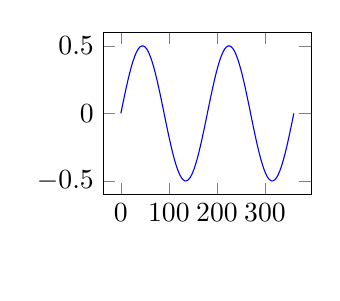
\begin{tikzpicture}[baseline=-1cm]\begin{axis}[width=120pt]
    \addplot+ [domain=0:360, samples=101, mark=none] {sin(2*x)/2};
  \end{axis}\end{tikzpicture}
\end{figure}
\begin{figure}[t!]\centering
  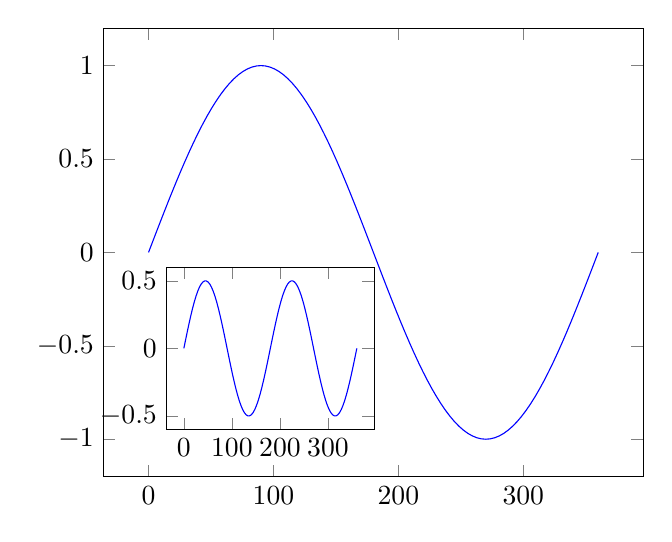
\begin{tikzpicture}\begin{axis}
    \addplot+ [domain=0:360, samples=101, mark=none] {sin(x)};
  \end{axis}\begin{axis}[width=120pt, at={(8mm,6mm)}]
    \addplot+ [domain=0:360, samples=101, mark=none] {sin(2*x)/2};
  \end{axis}\end{tikzpicture}
\end{figure}
\hfill  % so the figures move up
\end{document}